\graphicspath{{figures/design/}}
\chapter{Design}\label{ch:design}
Based on the acquired knowledge from \autoref{ch:intro} and \autoref{ch:data_anal} a design of an occlusion detection solution is made. This is implemented using Python3 with the Keras API working with Tensorflow.

This chapter gives an in-depth description of how the implementations are made and the theory behind them.\\

As stated in \autoref{ch:intro} the use of \gls{cnn}s in object detection is the highest performing solution in different benchmarks. Due to this it is chosen to utilise a \gls{cnn} to perform the occlusion detection of zebrafish. In the following description of \gls{cnn}s in general and of the implementation for object detection is presented.

\section{Convolutional Neural Networks (CNN)}
\begin{itemize}
	\item Overview
	\item Layer types
	\item Convolutional layers
\end{itemize}

As regular neural networks, \gls{cnn}s are made up of neurons which have learnable weights and biases. Each neuron in the network receives inputs, performs an operation on the input and passes the output on, either linearly or non-linearly, dependent on the design.\\

When a \gls{cnn} receives an input image and then transforms this through a series of hidden layers in the network. Each hidden layer consist of a set of neurons, and each neuron is fully connected to the neurons in the previous layer, but does not share any connections inside the layer. The last layer, the output layer, is a fully connected layer and represents the class scores. A \gls{cnn} has layers neurons arranged in three dimensions, namely: width, height, and depth. Already in the input an RGB image will have a depth of three due to the three colour channels. A small example of the \gls{cnn} architecture is shown in \autoref{fig:cnn_arch}.

\begin{figure}[H]
	\centering
	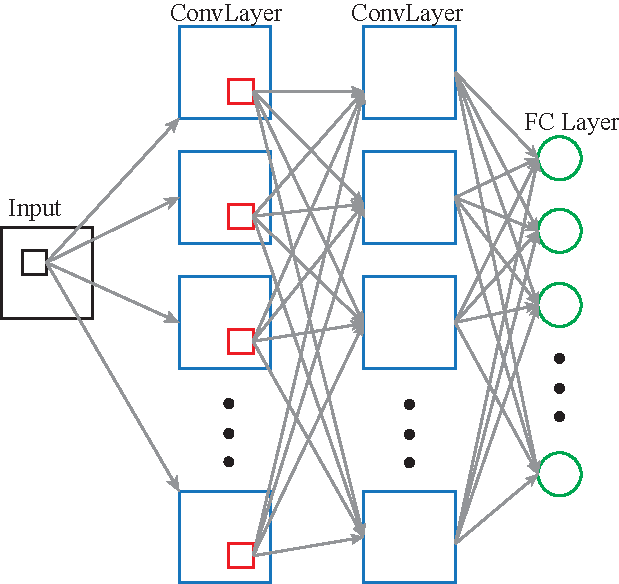
\includegraphics[width=0.6\textwidth]{cnn_arch}
	\caption{Example of a \gls{cnn} architecture}
	\label{fig:cnn_arch}
\end{figure}

\subsection{Layers}
A simple \gls{cnn} will often consist of a sequence of layers, in which each layer transforms one volume of activations to another through differentiable functions. The main layers used are; convolutional layer, pooling layer, and fully connected layer. These layers are presented in the following.

\subsubsection{Convolutional Layers}


\subsubsection{Pooling Layers}


\section{Faster R-CNN}
To be able to detect objects in a frame using a \gls{cnn} the Faster R-\gls{cnn} proposed by \cite{Ren2017} is used. The chosen solution model is the third iteration of the Region based Convolutional Neural Network by \cite{Girshick2014}. As the title proposes, the network is a region proposal based network, used for object detection in an image.

\subsection{Object Detection}
Object detection opposed to image classification aims to locate defined objects or instances in images, and often in images containing several objects to locate at the same time, whereas an image classification solution aims to classify one object in an image and recognise the the single object without any localisation.

\subsection{Region-based Convolutional Neural Network (R-CNN)} 
The model for the R-\gls{cnn} begins with a region search and then do the classification. This model uses \textit{Selective Search} which initialises regions in the image and then merge these with a hierarchical grouping. The final grouping is then a box containing the entire image. The regions are grouped in relation to colour space and similarity \citep{Girshick2014}.

The regions proposed are then fed into the \gls{cnn} which in this case extracts a $4096$ dimensional feature vector. From this feature vector a classification is done using an \gls{svm} for each class \citep{Girshick2014}. \autoref{fig:rcnn_flow} shows the steps in the R-\gls{cnn}.

%\begin{figure}[H]
%	\centering
%	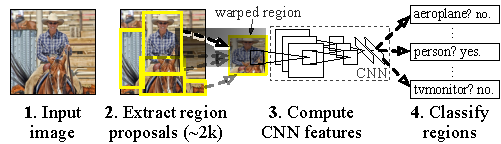
\includegraphics[width=0.8\textwidth]{rcnn_flow}
%	\caption{Simple flow diagram of the R-\gls{cnn} by \cite{Girshick2014}}
%	\label{fig:rcnn_flow}
%\end{figure}

The solution pre-trained on the ImageNet 2012 dataset and is fine tuned using an \gls{iou} greater than $0.5$ with the ground-truth boxes. At the time of development, \cite{Girshick2014} achieves a $62.4\%$ \gls{map} on the Pascal VOC 2012 dataset and $31.4\%$ \gls{map} on the ImageNet 2013 dataset, achieving top position on the leader boards for both datasets.

\subsection{Fast Region-based Convolutional Network (Fast R-CNN)}
The next iteration of the model by \cite{Girshick2015} is made to reduce time consumption due to the amount of models used to analyse all the regions proposed in the R-\gls{cnn}.

Instead of using the selective search on the entire image, a \gls{cnn} is used to extract features from the image, and the selective search is utilised to detect \gls{roi}s from the feature maps produced by the \gls{cnn} \citep{Girshick2015}.

\subsection{Faster Region-based Convolutional Network (Faster R-CNN)}
The third iteration of R-\gls{cnn} replaces the selective search with a \textit{Region Proposal Network (RPN)}, which is a network that generates regions proposals, predict bounding boxes and detects objects.

Here, once again, a \gls{cnn} is used to produce feature maps from the entire image and then uses the RPN to propose regions and feed these to a classifier.

The Faster R-\gls{cnn} outperforms the previous iterations in both accuracy and speed. Due to this, the Faster R-\gls{cnn} solution is chosen to utilise for an occlusion detection model.

\section{Occlusion Detection}
The implementation of the occlusion detection solution is done using the Keras API with Tensorflow, running on Google Colaboratory's Jupyter Notebook Environment.\\

Tanken med afsnittet, er at gå i dybden med alle dele af netværket hver for sig, hvorfor de er med og hvad de gør.

\subsection{Region Proposal Network}

\subsection{Intersection over Union}
